\section{图的基本概念}
\subsection{图的定义}
在给出图的定义之前,我们要引入两个谓词:
用\(\Ed(e,u,v)\)表示
\(e\)是以\(u\)为\DefineConcept{起点}、\(v\)为\DefineConcept{终点}的\DefineConcept{有向边}(directed edge),
用\(\Eu(e,u,v)\)表示
\(e\)是以\(u\)和\(v\)为\DefineConcept{端点}(endvertex)的\DefineConcept{无向边}(undirected edge).

\begin{definition}
%@see: 《离散数学》(邓辉文) P166
设\(V,E\)都是有限集.
\begin{itemize}
	\item 如果\(E\)的元素都是有向边,即\begin{equation*}
		(\forall e \in E)
		(\exists u,v \in V)
		[\Ed(e,u,v)],
	\end{equation*}
	则称“\((V,E)\)是一个\DefineConcept{有向图}(directed graph,简称 digraph)”.

	\item 如果\(E\)的元素都是无向边,即\begin{equation*}
		(\forall e \in E)
		(\exists u,v \in V)
		[\Eu(e,u,v)],
	\end{equation*}
	则称“\((V,E)\)是一个\DefineConcept{无向图}(undirected graph,简称 graph)”.

	\item 我们把有向图和无向图统称为\DefineConcept{图}(graph).
	% 没有讨论既含无向边,又含有向边的混合图

	\item 我们将有向边和无向边统称为\DefineConcept{边}(edge).
\end{itemize}
\end{definition}

\begin{definition}
%@see: 《离散数学》(邓辉文) P166 定义6-1
设\(G = (V,E)\)是图.
对于\(\forall v \in V\),
称“\(v\)是图\(G\)的一个\DefineConcept{顶点}(vertex)”,
或“\(v\)是图\(G\)的一个\DefineConcept{结点}(node)”.
\end{definition}

\begin{definition}
设\(G = (V,E)\)是有向图.
对于\(\forall e \in E\),
称为“\(e\)是图\(G\)的一条\DefineConcept{弧}(arc)”,
把\(e\)的起点\(v_1\)称为“\(e\)的\DefineConcept{弧尾}(tail)”,
把\(e\)的终点\(v_2\)称为“\(e\)的\DefineConcept{弧头}(head)”,
把\(v_1\)称为“\(v_2\)的\DefineConcept{前趋}”,
把\(v_2\)称为“\(v_1\)的\DefineConcept{后继}”.
\end{definition}
\begin{remark}
有向边的弧尾、弧头,无向边的两个端点,都可以是同一个顶点.
\end{remark}

\begin{definition}
%@see: 《Graph Theory》(Reinhard Diestel) P2
设图\(G = (V,E)\).
\begin{itemize}
	\item 把\(V\)称为“图\((V,E)\)的\DefineConcept{顶点集}”,记作\(V(G)\).
	\item 把\(E\)称为“图\((V,E)\)的\DefineConcept{边集}”,记作\(E(G)\).
\end{itemize}
\end{definition}
\begin{remark}
这里定义\(V(G),E(G)\)两个记号看似画蛇添足多此一举,
实际上它们起到了与\(\dom,\ran\)这两个记号类似的作用.
例如,对于图\(H = (W,F)\),我们可以断言\(V(H) = W,E(H) = F\).
另一方面,我们对于图及其顶点集、边集经常不作严格区分.
例如,我们会说顶点\(v \in G\),而非\(v \in V(G)\);
我们还会说边\(e \in G\),而非\(e \in E(G)\).
\end{remark}

\begin{definition}
%@see: 《离散数学》(邓辉文) P167 定义6-3
设\(G\)是图,
\(e\)是\(G\)的一条边,
\(u,v\)是\(G\)的两个顶点.
如果\begin{equation*}
	\Ed(e,u,v)
	\lor
	\Eu(e,u,v),
\end{equation*}
则称“\(e\)与\(u,v\)是\DefineConcept{关联的}(incident)”,
或“\(u\)和\(v\)是\(e\)的\DefineConcept{关联顶点}%
(\(u\) and \(v\) are \emph{incident vertices} of \(e\))”.
\end{definition}

\begin{definition}
%@see: 《离散数学》(邓辉文) P167 定义6-2
设\(u,v\)是图\((V,E)\)的两个顶点.
\begin{itemize}
	\item 如果\begin{equation*}
		(\exists e \in E)
		[
			\Eu(e,u,v)
			\lor
			\Ed(e,u,v)
		],
	\end{equation*}
	则称“\(u\)与\(v\) \DefineConcept{邻接}%
	(\(u\) is \emph{adjacent to} \(v\),
	\(u\) and \(v\) are \emph{adjacent},
	\(u\) and \(v\) are \emph{neighbours})”;

	%@see: 《Graph Theory》(Reinhard Diestel) P3
	\item 否则称“\(u\)与\(v\) \DefineConcept{独立}%
	(\(u\) and \(v\) are \emph{independent})”.
\end{itemize}
\end{definition}

\begin{definition}
%@see: 《离散数学》(邓辉文) P167
设\(e,f\)是无向图\((V,E)\)的两条边,\(e \neq f\).
\begin{itemize}
	\item 若\(e,f\)有公共端点,即\begin{equation*}
		(\exists u,v,w)
		[
			\Eu(e,u,v)
			\land
			\Eu(f,v,w)
		],
	\end{equation*}
	则称“\(e\)和\(f\)是\DefineConcept{邻接的}%
	(\(e\) and \(f\) are \emph{adjacent})”;

	%@see: 《Graph Theory》(Reinhard Diestel) P3
	\item 否则,称“\(e\)与\(f\) \DefineConcept{独立}%
	(\(e\) and \(f\) are \emph{independent})”.
\end{itemize}
\end{definition}

\begin{definition}
%@see: 《Graph Theory》(Reinhard Diestel) P3
设图\((V,E)\).
\begin{itemize}
	\item 如果\(W \subseteq V\),且\begin{equation*}
		(\forall v_1,v_2 \in W)
		\left[\text{$v_1$与$v_2$独立}\right],
	\end{equation*}
	则称“\(W\)是独立的(\(W\) is \emph{independent})”,
	或称“\(W\)是稳定的(\(W\) is \emph{stable})”.

	\item 如果\(F \subseteq E\),且\begin{equation*}
		(\forall e_1,e_2 \in F)
		\left[\text{$e_1$与$e_2$独立}\right],
	\end{equation*}
	则称“\(F\)是独立的(\(F\) is \emph{independent})”,
	或称“\(F\)是稳定的(\(F\) is \emph{stable})”.
\end{itemize}
\end{definition}

\subsection{图的图形表示}
对于任意一个图\(G\),
我们总可以将它绘制在欧氏空间\(\mathbb{R}^3\)中:
首先将\(G\)的不同顶点画在不同位置;
接下来按照边与顶点的关联关系,用曲线段或有向曲线段连接顶点.
这样画出的图形,
称为“图\(G\)的\DefineConcept{图形表示}”.
\begin{remark}
图具有拓扑不变性质 ---
这就是说,我们讨论的图,不但与顶点的位置无关,而且与边的形状和长短也无关
--- 我们关注的,只有顶点与顶点之间是否通过某几条边直接或间接相连.
\end{remark}

\begin{figure}[hbt]
%@see: 《离散数学》(邓辉文) P165 图6-1(b)
	\centering
	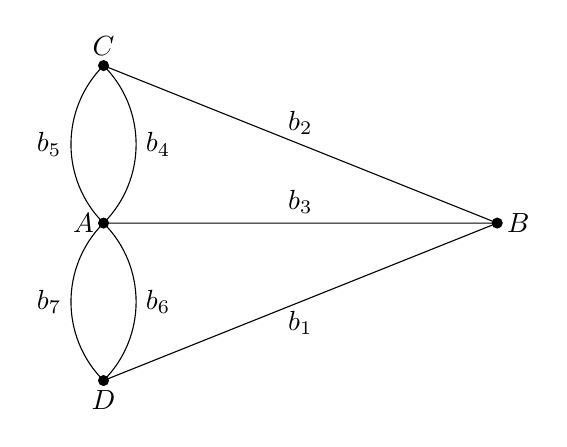
\begin{tikzpicture}
		\fill(0,0)coordinate(A)circle(2pt)node[left]{$A$}
			(5,0)coordinate(B)circle(2pt)node[right]{$B$}
			(0,2)coordinate(C)circle(2pt)node[above]{$C$}
			(0,-2)coordinate(D)circle(2pt)node[below]{$D$};
		\draw(A)--(B)node[midway,above]{$b_3$}
			(A)to[out=45,in=-45]node[midway,right]{$b_4$}(C)
			(A)to[out=135,in=-135]node[midway,left]{$b_5$}(C)
			(A)to[out=-45,in=45]node[midway,right]{$b_6$}(D)
			(A)to[out=-135,in=135]node[midway,left]{$b_7$}(D)
			(C)--(B)node[midway,above]{$b_2$}--(D)node[midway,below]{$b_1$};
	\end{tikzpicture}
	\caption{七桥问题}
	\label{figure:图论.七桥问题}
\end{figure}

如\cref{figure:图论.七桥问题} 所示,
令\begin{equation*}
	V = \{A,B,C,D\},
	\qquad
	E = \{\AutoTuple{b}{7}\},
\end{equation*}
则\((V,E)\)是一个无向图,
\(A,B,C,D\)都是这个图的顶点,
\(\AutoTuple{b}{7}\)都是这个图的边,
\(b_1\)的端点是\(B,D\),
\(b_2\)的端点是\(B,C\),
\(b_3\)的端点是\(A,B\),
\(b_4\)和\(b_5\)的端点都是\(A,C\),
\(b_6\)和\(b_7\)的端点都是\(A,D\).

\begin{example}[过河问题]
%@see: 《离散数学》(邓辉文) P169 习题6.1 6.(过河问题)
某人挑一担菜,带着一条狼和一只羊,要从河的一边到另一边.
由于渡船太小,只能带狼、羊、菜中的一样过河.
当人不在场时,狼要吃羊,羊要吃菜.
请尝试建立图模型,给出解决方法.
\begin{solution}
不妨忽略渡船在河中航行的时间,
那么只要人位于出发地,就不会位于目的地,反之亦然,狼、羊、菜同理,
可以看出人、狼、羊、菜各自所处位置可以用\(0,1\)两个数字表示,
用\(0\)表示“在出发地”,用\(1\)表示“在目的地”.
于是我们可以用4位数字,从高位到低位,依次表示人、狼、羊、菜的状态.
由题意可知,把人、狼、羊、菜看作一个整体,总的状态数是\(2^4 = 16\)种,
其中\(1100,1001,1000,0111,0110,0011\)这6种状态是非法状态,
无法避免狼吃羊或羊吃菜;
在去掉这6种非法状态以后,
合法状态就只剩下\(1111,1110,1101,1011,1010,0101,0100,0010,0001,0000\)这10种.

接下来,我们需要确定各个状态是否可以相互转化.
因为每次只能带狼、羊、菜种的一样过河,
所以每次状态转移都有代表人的数位和狼、羊、菜种某一样对应的数位发生翻转.
于是我们可以得到如下的状态图:
\begin{center}
	\tikzset{every state/.style={minimum size=1cm}}
	% requires `\usetikzlibrary{automata}'
	\begin{tikzpicture}[node distance=2cm]
		\node[state](S00){0000};
		\node[state](S10)[below of=S00]{1010};
		\node[state](S02)[right of=S10]{0010};
		\node[state](S11)[below of=S02]{1011};
		\node[state](S14)[above of=S02]{1110};
		\node[state](S04)[right of=S14]{0100};
		\node[state](S13)[below of=S04]{1101};
		\node[state](S01)[below of=S13]{0001};
		\node[state](S05)[right of=S13]{0101};
		\node[state](S15)[below of=S05]{1111};

		\draw(S00)--(S10)--(S02)--(S14)--(S04)--(S13)--(S01)--(S11)--(S02)
			(S13)--(S05)--(S15);
	\end{tikzpicture}
\end{center}

从图中可以看出,
不论是沿着\(0000,\allowbreak1010,\allowbreak0010,\allowbreak1110,\allowbreak0100,\allowbreak1101,\allowbreak0101,\allowbreak1111\)这条路径
(人羊同行,人独自返回,人狼同行,人羊返回,人菜同行,人独自返回,人羊同行),
还是沿着\(0000,\allowbreak1010,\allowbreak0010,\allowbreak1011,\allowbreak0001,\allowbreak1101,\allowbreak0101,\allowbreak1111\)这条路径
(人羊同行,人独自返回,人菜同行,人羊返回,人狼同行,人独自返回,人羊同行),
均可从初始状态\(0000\)抵达目标状态\(1111\).
\end{solution}
\end{example}

\subsection{图中元素的计数,图的分类}
\begin{definition}
%@see: 《Graph Theory》(Reinhard Diestel) P2
设图\(G = (V,E)\),
定义:\begin{gather*}
	\abs{G} \defeq \card V, \\
	\norm{G} \defeq \card E.
\end{gather*}
把\(\abs{G}\)称为“\(G\)的\DefineConcept{阶数}(order)”
或“\(G\)的\DefineConcept{顶点数}”.
把\(\norm{G}\)称为“\(G\)的\DefineConcept{边数}”.
\end{definition}

\begin{definition}
%@see: 《离散数学》(邓辉文) P166
有\(n\)个顶点的图,
称为 \DefineConcept{\(n\)阶图}.
\end{definition}

\begin{definition}
%@see: 《离散数学》(邓辉文) P166
有\(n\)个顶点、\(m\)条边(弧)的图,
称为 \DefineConcept{\((n,m)\)图}.
\end{definition}

\begin{definition}
%@see: 《离散数学》(邓辉文) P167
若图\(G = (V,E)\)
满足\(V = \emptyset\),
则称“\(G\)是\DefineConcept{空图}(empty graph)”,
记作\(\emptyset\).
\end{definition}

\begin{definition}
%@see: 《离散数学》(邓辉文) P167
若图\(G = (V,E)\)
满足\(V \neq \emptyset,E = \emptyset\),
则称“\(G\)是\DefineConcept{零图}(discrete graph)”.
特别地,\(k\)阶零图记作\(N_k\),
仅有一个顶点的零图称为\DefineConcept{平凡图}(trivial graph).
\end{definition}

\begin{definition}
%@see: 《离散数学》(邓辉文) P171 习题6.2 4.
将有向图\(G\)的有向边都换成无向边,
得到的无向图\(H\)称为“\(G\)的\DefineConcept{基础图}”.
\end{definition}

\begin{definition}
%@see: 《离散数学》(邓辉文) P167
设边\(e\)与顶点\(u,v\)关联.
如果\(u = v\),
则称“\(e\)是一条\DefineConcept{自环}(loop)”.
\end{definition}

如\cref{figure:图论.带有自环的无向图} 所示,顶点\(v_2\)有\(e_1,e_2\)两个自环.

\begin{figure}[hbt]
%@see: 《离散数学》(邓辉文) P166 图6-4(a)
%@see: 《离散数学》(邓辉文) P166 图6-9(a)
	\centering
	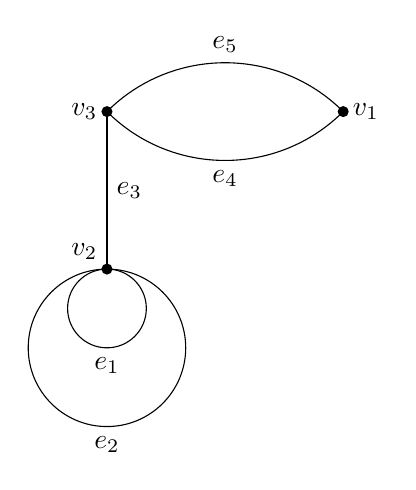
\begin{tikzpicture}
		\fill(3,2)coordinate(v1)node[right]{$v_1$}circle(2pt);
		\fill(0,0)coordinate(v2)node[above left]{$v_2$}circle(2pt);
		\fill(0,2)coordinate(v3)node[left]{$v_3$}circle(2pt);
		\draw(v2)++(0,-.5)circle(.5) (v2)++(0,-1)node[below]{$e_1$};
		\draw(v2)++(0,-1)circle(1) (v2)++(0,-2)node[below]{$e_2$};
		\draw(v2)--(v3)node[midway,right]{$e_3$};
		\draw(v1)to[out=-135,in=-45]node[midway,below]{$e_4$}(v3);
		\draw(v1)to[out=135,in=45]node[midway,above]{$e_5$}(v3);
	\end{tikzpicture}
	\caption{}
	\label{figure:图论.带有自环的无向图}
\end{figure}

\begin{definition}
%@see: 《离散数学》(邓辉文) P167
设边\(e_1\)与顶点\(u_1,v_1\)关联,
边\(e_2\)与顶点\(u_2,v_2\)关联.
如果\(u_1 = u_2,
v_1 = v_2\),
则称“\(e_1,e_2\)是一组\DefineConcept{多重边}(multiple edges)”,
或称“\(e_1,e_2\)是一组\DefineConcept{平行边}”.
\end{definition}

如\cref{figure:图论.七桥问题} 所示,
\(b_4,b_5\)是一组多重边,
\(b_6,b_7\)是另一组多重边.

\begin{definition}
%@see: 《离散数学》(邓辉文) P167
给定顶点\(u_0,v_0\),
其多重边的边数\begin{equation*}
	\card\Set{
		e \in E
		\given
		\text{$e$与$u_0,v_0$关联}
	}
\end{equation*}
称为“\(u_0\)与\(v_0\)之间的边的\DefineConcept{重数}(multiplicity)”.
\end{definition}

如\cref{figure:图论.七桥问题} 所示,
顶点\(A,C\)之间的边的重数为\(2\).

\subsection{简单图,完全图,补图}
\begin{definition}
%@see: 《离散数学》(邓辉文) P167 定义6-4
设图\(G\)既没有自环,也没有多重边,
则称“\(G\)是\DefineConcept{简单图}(simple graph)”.
\end{definition}

如\cref{figure:图论.彼得森图} 所示,
彼得森图是简单图.

\begin{definition}
%@see: 《离散数学》(邓辉文) P167 定义6-5
如果\(n\)阶简单无向图\(G\)中任意一个顶点都与其余\(n-1\)个顶点邻接,
则称“\(G\)是\(n\)阶\DefineConcept{完全无向图}(complete graph)”,
记作\(K_n\).
\end{definition}

\begin{figure}[hbt]
%@see: 《离散数学》(邓辉文) P167 图6-5
	\centering
	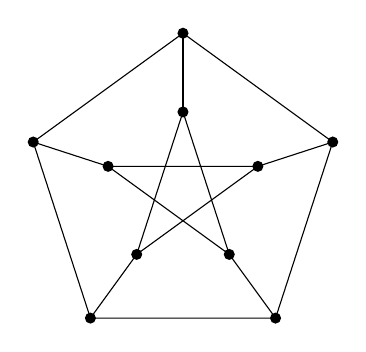
\begin{tikzpicture}
		\foreach \j in {0,...,4} {
			\fill({cos(\j*72+90)},{sin(\j*72+90)})coordinate(A\j)circle(2pt);
			\fill({2*cos(\j*72+90)},{2*sin(\j*72+90)})coordinate(B\j)circle(2pt);
			\draw(A\j)--(B\j);
		}
		\draw(A0)--(A2) (A1)--(A3) (A2)--(A4) (A3)--(A0) (A4)--(A1);
		\draw(B0)--(B1)--(B2)--(B3)--(B4)--(B0);
	\end{tikzpicture}
	\caption{彼得森图}
	\label{figure:图论.彼得森图}
\end{figure}

\begin{figure}[hbt]
%@see: 《离散数学》(邓辉文) P168 图6-6
	\centering
	\def\subwidth{.3\linewidth}
	\begin{subfigure}[b]{\subwidth}
		\centering
		\def\n{3}  % 控制顶点数
		\def\b{90}  % 控制图像绕其几何中心旋转的角度(相位)
		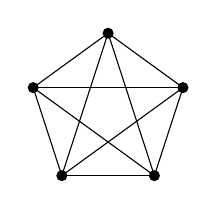
\begin{tikzpicture}
			\pgfmathsetmacro{\m}{\n-1}
			\pgfmathsetmacro{\a}{360/\n}
			\foreach \j in {0,...,\m} {
				\fill({cos(\j*\a+\b)},{sin(\j*\a+\b)})coordinate(A\j)circle(2pt);
			}
			\foreach \j in {0,...,\m} {
				\foreach \k in {0,...,\m} {
					\ifnum\j<\k\relax
						\draw(A\j)--(A\k);
					\fi
				}
			}
		\end{tikzpicture}
		\caption{\n 阶完全无向图\(K_\n\)}
	\end{subfigure}~\begin{subfigure}[b]{\subwidth}
		\centering
		\def\n{4}
		\def\b{45}
		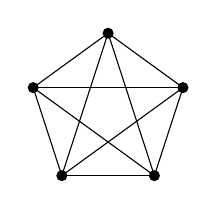
\begin{tikzpicture}
			\pgfmathsetmacro{\m}{\n-1}
			\pgfmathsetmacro{\a}{360/\n}
			\foreach \j in {0,...,\m} {
				\fill({cos(\j*\a+\b)},{sin(\j*\a+\b)})coordinate(A\j)circle(2pt);
			}
			\foreach \j in {0,...,\m} {
				\foreach \k in {0,...,\m} {
					\ifnum\j<\k\relax
						\draw(A\j)--(A\k);
					\fi
				}
			}
		\end{tikzpicture}
		\caption{\n 阶完全无向图\(K_\n\)}
	\end{subfigure}~\begin{subfigure}[b]{\subwidth}
		\centering
		\def\n{5}
		\def\b{90}
		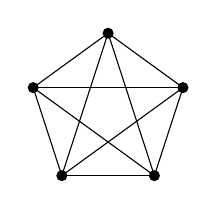
\begin{tikzpicture}
			\pgfmathsetmacro{\m}{\n-1}
			\pgfmathsetmacro{\a}{360/\n}
			\foreach \j in {0,...,\m} {
				\fill({cos(\j*\a+\b)},{sin(\j*\a+\b)})coordinate(A\j)circle(2pt);
			}
			\foreach \j in {0,...,\m} {
				\foreach \k in {0,...,\m} {
					\ifnum\j<\k\relax
						\draw(A\j)--(A\k);
					\fi
				}
			}
		\end{tikzpicture}
		\caption{\n 阶完全无向图\(K_\n\)}
	\end{subfigure}
	\caption{完全图}
\end{figure}

\begin{proposition}
\(n\)阶完全无向图\(K_n\)的边数为
\(n(n-1)/2\).
\end{proposition}

\begin{definition}
设\(G\)是\(n\)阶简单有向图.
若\(G\)中任意顶点都与其余\(n-1\)个顶点邻接,
则称“\(G\)是\(n\)阶\DefineConcept{完全有向图}”.
\end{definition}

我们将完全无向图、完全有向图统称为\DefineConcept{完全图}.

\begin{definition}
%@see: 《离散数学》(邓辉文) P171 习题6.2 4.
基础图是完全图的有向图,称为\DefineConcept{竞赛图}.
% 另一种表述方式:
% 将\(n\)阶完全无向图\(K_n\)的边
% 任意加一个方向所得到的有向图
% 称为\(n\)阶\DefineConcept{竞赛图}.
\end{definition}


\begin{definition}
%@see: 《离散数学》(邓辉文) P168 定义6-6
设\(G\)是\(n\)阶简单无向图.
由\(G\)的所有顶点
以及能使\(G\)成为\(K_n\)需要添加的边构成的图,
称为“\(G\)的\DefineConcept{补图}(complementary graph)”,
记为\(\overline{G}\).
\end{definition}

\begin{figure}[hbt]
%@see: 《离散数学》(邓辉文) P168 图6-6
%@see: 《离散数学》(邓辉文) P173 图6-16
	\centering
	\def\subwidth{.3\linewidth}
	\begin{subfigure}[b]{\subwidth}
		\centering
		\def\n{5}
		\def\b{90}
		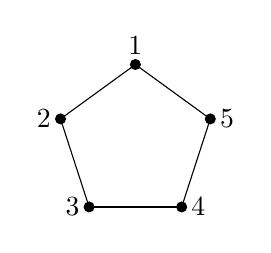
\begin{tikzpicture}
			\pgfmathsetmacro{\m}{\n-1}
			\pgfmathsetmacro{\a}{360/\n}
			\foreach \j in {0,...,\m} {
				\fill({cos(\j*\a+\b)},{sin(\j*\a+\b)})coordinate(A\j)circle(2pt);
				\draw({cos(\j*\a+\b)},{sin(\j*\a+\b)})
					--({cos((\j+1)*\a+\b)},{sin((\j+1)*\a+\b)});
			}
			\draw(A0)node[above]{1}
				(A1)node[left]{2}
				(A2)node[left]{3}
				(A3)node[right]{4}
				(A4)node[right]{5};
		\end{tikzpicture}
		\caption{}
		\label{figure:图论.补图.原图1}
	\end{subfigure}~\begin{subfigure}[b]{\subwidth}
		\centering
		\def\n{5}
		\def\b{90}
		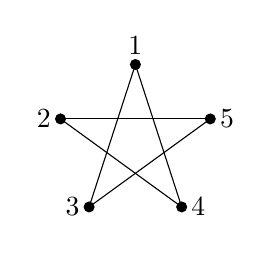
\begin{tikzpicture}
			\pgfmathsetmacro{\m}{\n-1}
			\pgfmathsetmacro{\a}{360/\n}
			\foreach \j in {0,...,\m} {
				\fill({cos(\j*\a+\b)},{sin(\j*\a+\b)})coordinate(A\j)circle(2pt);
				\draw({cos(\j*\a+\b)},{sin(\j*\a+\b)})
					--({cos((\j+2)*\a+\b)},{sin((\j+2)*\a+\b)});
			}
			\draw(A0)node[above]{1}
				(A1)node[left]{2}
				(A2)node[left]{3}
				(A3)node[right]{4}
				(A4)node[right]{5};
		\end{tikzpicture}
		\caption{}
		\label{figure:图论.补图.补图1}
	\end{subfigure}
	\caption{}
\end{figure}

\cref{figure:图论.补图.原图1} 中的图
与\cref{figure:图论.补图.补图1} 中的图
互为补图.

\begin{proposition}
%@see: 《离散数学》(邓辉文) P168
对于任意顶点\(u,v\),
若\(u\)和\(v\)在\(G\)中不邻接,
则\(u\)和\(v\)在\(\overline{G}\)中邻接;
若\(u\)和\(v\)在\(G\)中邻接,
则\(u\)和\(v\)在\(\overline{G}\)中不邻接.
\end{proposition}

\begin{example}
%@see: 《离散数学》(邓辉文) P169 习题6.1 9.
设\(n\)阶简单无向图\(G\)有\(m\)条边,
求\(G\)的补图\(\overline{G}\)的边数.
\begin{solution}
因为\(n\)阶完全图的边数是\(\frac{n(n-1)}2\),
所以\(G\)的补图\(\overline{G}\)的边数为\(\frac{n(n-1)}2-m\).
\end{solution}
\end{example}
